\subsection{Defining Work on a Gas}
As you may remember from the previous unit, work is generally defined as
\begin{equation}
    W = \int_{x_1}^{x_2} Fdx
\end{equation}
However, in thermodynamics we don't have position or force as variables to work with. Instead, we have pressure and volume. So, we need to find a way to define force and position in terms of pressure and volume. Starting with force, I can say that $F = PA$, so substituting that into the equation we get
\begin{equation*}
    W = \int_{x_1}^{x_2} PAdx
\end{equation*}
The product of area and distance is volume (Think of a cube. What's the area of on of the cube's faces times the length of its side?). So, since dx is a tiny displacement, which ultimately is a length, Adx is a tiny change in volume! Therefore:
\begin{equation*}
    W = \int_{V_1}^{V_2} PdV
\end{equation*}
However, there's one more issue with this. The way I've defined work so far was based on the definition of the amount of work done \textbf{by} a system on another system. We want the amount of work done \textbf{on} the system. Due to conservation of energy, I can just throw a negative sign in front to get
\begin{equation}
    W = -\int_{V_1}^{V_2} PdV
\end{equation}
This is the proper definition of the work done on a gas. One thing to be careful of here; It looks like the pressure $P$ is just a constant I can take out of the integral. This is only the case if the pressure is \textit{actually a constant over the entire process}. Otherwise, the pressure really is a function of volume, and so we keep it inside the integral; to be extra clear that the pressure is changing as a function of volume, we should write the equation as:
\begin{equation}
    \label{eqn:(16)}
    W = -\int_{V_1}^{V_2} P(V)dV
\end{equation}
The below diagram illustrates gas in a box with a piston, and shows the work done by the gas (because it's easier to draw):
\begin{center}
    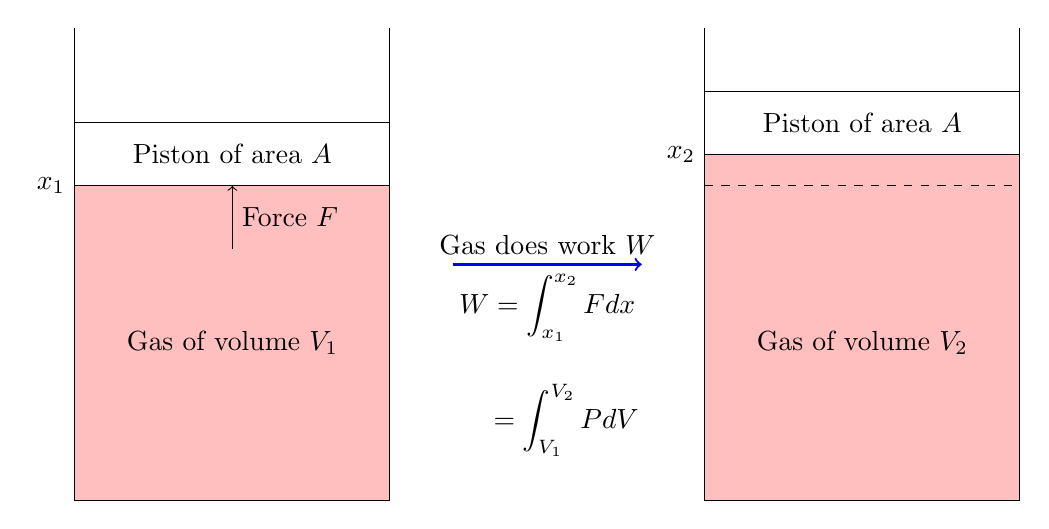
\begin{tikzpicture}[scale=4]
    \filldraw[fill=pink, draw = black] (0,0) rectangle (1,1);
    \draw[black] (0,1) rectangle (1,1.2);
    \draw (0,1.2) -- (0,1.5);
    \draw (1,1.2) -- (1,1.5);
    \draw[->] (0.5,0.8) -- (0.5,1);
    \node[right] at (0.5,0.9) {Force $F$};
    \node[left] at (0,1) {$x_1$};
    \draw (0.5,0.5) node {Gas of volume $V_1$};
    \draw (0.5, 1.1) node {Piston of area $A$};
    \draw[->, blue, thick] (1.2,0.75) -- (1.8, 0.75);
    \node[above] at (1.5,0.75) {Gas does work $W$};
    \node[below] at (1.5,0.75) {$\displaystyle W = \int_{x_1}^{x_2} Fdx$};
    \node[below] at (1.5,0.4) {$\displaystyle \phantom{W }=  \int_{V_1}^{V_2} PdV$};
    \filldraw[fill=pink, draw = black] (2,0) rectangle (3,1.1);
    \draw[black] (2,1.1) rectangle (3,1.3);
    \draw[dashed] (2,1) -- (3,1);
    \draw (2,1.2) -- (2,1.5);
    \draw (3,1.2) -- (3,1.5);
    \node[left] at (2,1.1) {$x_2$};
    \draw (2.5,0.5) node {Gas of volume $V_2$};
    \draw (2.5, 1.2) node {Piston of area $A$};
    \end{tikzpicture}
\end{center}
